
\subsection{Measurement Method}
To get more accurate performance measurement result, we design the experiment very carefully. First, we assume that Dropbox API will compare user data with what the already had in the cloud before the API actually upload the file. It is reasonable for them to do so to avoid massive redundant uploading bandwidth. However, for our measurement, this is not a good property because the upload speed will be much faster than it should be after the first upload action. To avoid this kind of situation, we generate a new random file with a random file name from system random source /dev/urandom each time before we upload it. Since each time both the file name and the content is different, the Dropbox API has no chance to compare the data before upload. Then we can measure the actual time consuming during upload/download progress.

Second, as the suggestion from Professor Alex C. Snoeren, we also scramble the order of uploading and downloading tasks. Sequential uploading or downloading files with the same file size could not ignore the fact that the network between sysnet clusters and Dropbox is not always stable. The file-transfer-speed statistics collected could be affected by the current network condition. We generate a random test order for different file size to avoid this problem. In the following evaluation, we run each test at least 100 times and get the average data from the results.

Third, we run the test with different Dropbox accounts and different sysnet cluster machines. Keep running a script that uploads and downloads small files continuously maybe will soon be noticed by Dropbox servers. To avoid the possible limitation on file-transfer-speed by the service providers, we switch the account randomly and test the script on different machines with different IP address.

\subsection{Dropbox Overhead and Performance}
We first found that the Dropbox Java API has a huge overhead on each uploading and downloading operation. This overhead dramatically slows down the performance of Trusted Bridge. We do not have enough time to implement the API by pure HTTP requests, so we decide to test the Dropbox API overhead and assume that we could minimize this overhead in the future with better implementation. The method to estimate the overhead is to generate a empty file by linux touch command. The file will be created with 0 Byte disk occupation and online contains metadata information. The average upload time for one single upload task with one empty file is 3.45 seconds. The average download time for the same file just uploaded is 3.12 second. 

To test the general performance of Dropbox uploading and downloading performance, we generate a series of random files with size 1Byte, 1KB, ad 1MB to 128MB. The result is shown in Figure~\ref{fig:dropbox_speed}. All the statistics are in Mbps unit. Averagely the download speed is a little faster than upload speed. The difference is about 3Mbps, which is not so significant. The interesting fact here is the performance is very bad when uploading or downloading small files. The speed is converged at about file size 4M to 8M. According to this phenomenon, we believe that Dropbox API will do file upload and download in chunk. The chunk size should be around 4M to 8M. 

\begin{figure}[ht]
\centering
%\includegraphics[width=3.5in]{pics/system_architecture.eps}
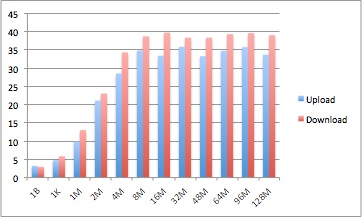
\includegraphics[width=3.5in]{pics/dropbox_speed.png}
\caption{Dropbox upload and download performance}
\label{fig:dropbox_speed}
\end{figure}

\subsection{Trusted Bridge Performance}
Figure~\ref{fig:upload_line} shows the upload speed comparison between Dropbox and Trusted Bridge server. The performance of Trusted Bridge on uploading small files are significantly worse than using pure Dropbox API. Figure~\ref{fig:download_line} shows the download speed comparison. Very similar pattern is showed in the graph as uploading test. The best performance lose is 9.57\% with the file size 128M. The worst performance lose for uploading, however, is 97\% with file size smaller than 4M. The best performance lose is 8.62\% with the file size 128M. The worst performance lose for uploading, however, is 96\% with file size smaller than 4M. 

The main reason of the performance degradation is that we separate each uploaded files into 32 pieces and upload them through Dropbox API one by one. The Dropbox API overhead will dramatically affect on our system performance. We believe we could find a better way to handle external cloud storage, so here we assume that we could remove the effect of the Dropbox uploading and downloading overhead. Because each file needs 32 upload or download task, we compare the speed performance between Trusted Bridge and Dropbox uploading or downloading the same actual file size. For example, uploading 128M file to Trusted Bridge server compare to uploading 4M file to Dropbox. The result is shown in Figure~\ref{fig:upload_bar} and Figure~\ref{fig:download_bar}. In this comparison, we could found that Trusted Bridge server only lose averagely 8.2\% on uploading and 9.7\% on downloading speed. This result shows the overall partitioning and assembling performance do not degrade the system performance too much. With our robust file scrambling algorithm, the user could save their files in their own cloud storage without losing the privacy. What he or she scarifies is just about 8 to 10 percent performance lose, which could hardly be noticed especially when user run our service in background like how current Dropbox or Google Drive works.


\begin{figure}[ht]
\centering
%\includegraphics[width=3.5in]{pics/system_architecture.eps}
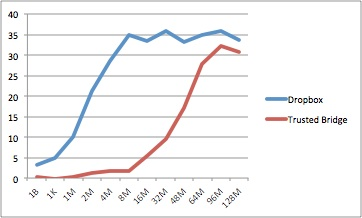
\includegraphics[width=3.5in]{pics/upload_line.png}
\caption{Upload speed comparison}
\label{fig:upload_line}
\end{figure}

\begin{figure}[ht]
\centering
%\includegraphics[width=3.5in]{pics/system_architecture.eps}
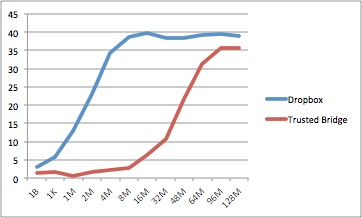
\includegraphics[width=3.5in]{pics/download_line.png}
\caption{Download speed comparison}
\label{fig:download_line}
\end{figure}

\begin{figure}[ht]
\centering
%\includegraphics[width=3.5in]{pics/system_architecture.eps}
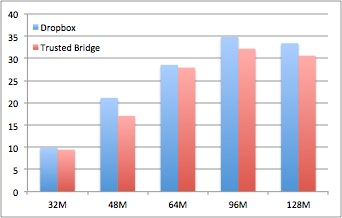
\includegraphics[width=3.5in]{pics/upload_bar.png}
\caption{Calibrated upload speed comparison. The file size here is the size uploaded to Trusted BRidge server}
\label{fig:upload_bar}
\end{figure}

\begin{figure}[ht]
\centering
%\includegraphics[width=3.5in]{pics/system_architecture.eps}
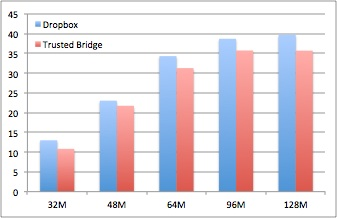
\includegraphics[width=3.5in]{pics/download_bar.png}
\caption{Calibrated download speed comparison. The file size here is the size downloaded from Trusted BRidge server}
\label{fig:download_bar}
\end{figure}